% Drawing 154/04-3 -- folder 154, batch 04, archive page 65 (PDF page 66).
% Transcription: figure : deux pseudo-droites orange se croisant sur une droite vert foncé marquée $s$ (?) à son extrémité ; au-dessous, une rangée de points noirs, hachurée de vert clair au-dessus (marqué $\omega$) et de vert foncé au-dessous (marqué $\omega'$) ; plus bas, une droite vert clair fléchée marquée $\omega_D$. « continuation » et « immersion » sont soulignés
% Kind: two pseudolines crossing on a line, hatched bands with orientations. Method 2 (schematic redraw from the facsimile). Status: ok.
% Notes: Two orange pseudolines crossing on a dark green line (marked at its right end by a letter, s (?) in the transcription, an arrowhead-like « D » on the facsimile); below, a row of black points, hatched in light green above (marked omega) and in dark green below (marked omega'); lower down, a light green arrowed line marked omega_D. Read from the page view.
% Coordinates: 1 unit = 1 mm = 1/100 of the crop width (bbox in page fractions: [0.583, 0.153, 0.81, 0.262]).
% Redrawn by Claude (claude-opus-5-5), issue #73, 2026-11-07; not checked by a human; not compiled (no TeX in the session).
% Rights: reproduces part of the work -- behind RENDER_TRANSCRIPTS, never published by itself.
\documentclass[tikz,border=3pt]{standalone}
\usepackage{amsmath,amssymb}
\usetikzlibrary{patterns,arrows.meta}
\tikzset{Or/.style={orange!90!black}, Ye/.style={yellow!80!orange}, Lg/.style={green!60!black!70}, Dg/.style={green!45!black}, Br/.style={brown!80!black}, Rd/.style={red!85!black}, Bl/.style={blue!70!black}, Gy/.style={black!40}, pencil/.style={black!45}, struck/.style={black!35}, mark/.style={circle,draw,inner sep=1.3pt}, pt/.style={circle,fill,inner sep=0.9pt}, opt/.style={circle,draw,fill=white,inner sep=1.1pt}}
\begin{document}
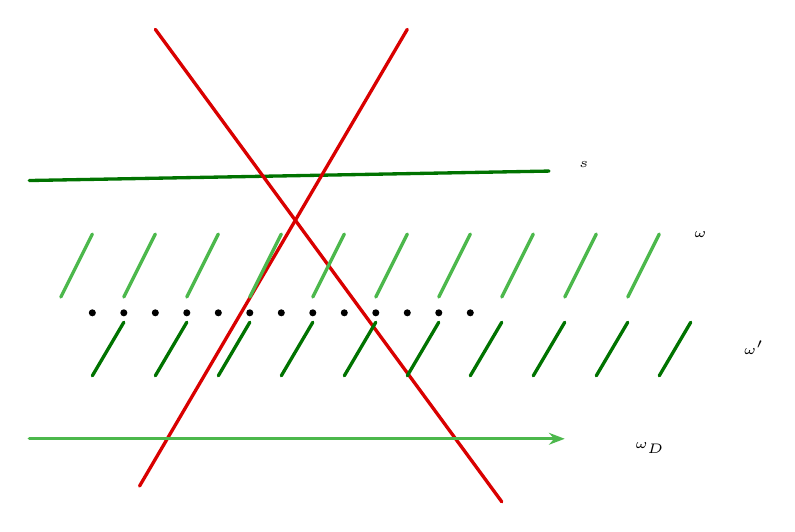
\begin{tikzpicture}[x=1mm,y=1mm,line cap=round,line join=round,font=\scriptsize]
\draw[Dg,very thick] (4,-23.2) -- (70,-22);
\node[inner sep=1pt] at (74.4,-21.2) {\tiny $s$};
\draw[Rd,very thick] (20,-4) -- (64,-64);
\draw[Rd,very thick] (52,-4) -- (18,-62);
\node[pt] at (12,-40) {};
\node[pt] at (16,-40) {};
\node[pt] at (20,-40) {};
\node[pt] at (24,-40) {};
\node[pt] at (28,-40) {};
\node[pt] at (32,-40) {};
\node[pt] at (36,-40) {};
\node[pt] at (40,-40) {};
\node[pt] at (44,-40) {};
\node[pt] at (48,-40) {};
\node[pt] at (52,-40) {};
\node[pt] at (56,-40) {};
\node[pt] at (60,-40) {};
\draw[Lg,very thick] (8,-38) -- (12,-30);
\draw[Lg,very thick] (16,-38) -- (20,-30);
\draw[Lg,very thick] (24,-38) -- (28,-30);
\draw[Lg,very thick] (32,-38) -- (36,-30);
\draw[Lg,very thick] (40,-38) -- (44,-30);
\draw[Lg,very thick] (48,-38) -- (52,-30);
\draw[Lg,very thick] (56,-38) -- (60,-30);
\draw[Lg,very thick] (64,-38) -- (68,-30);
\draw[Lg,very thick] (72,-38) -- (76,-30);
\draw[Lg,very thick] (80,-38) -- (84,-30);
\draw[Dg,very thick] (12,-48) -- (16,-41.2);
\draw[Dg,very thick] (20,-48) -- (24,-41.2);
\draw[Dg,very thick] (28,-48) -- (32,-41.2);
\draw[Dg,very thick] (36,-48) -- (40,-41.2);
\draw[Dg,very thick] (44,-48) -- (48,-41.2);
\draw[Dg,very thick] (52,-48) -- (56,-41.2);
\draw[Dg,very thick] (60,-48) -- (64,-41.2);
\draw[Dg,very thick] (68,-48) -- (72,-41.2);
\draw[Dg,very thick] (76,-48) -- (80,-41.2);
\draw[Dg,very thick] (84,-48) -- (88,-41.2);
\node[inner sep=1pt] at (89.2,-30) {\tiny $\omega$};
\node[inner sep=1pt] at (96,-44.4) {\tiny $\omega'$};
\draw[Lg,very thick,-{Stealth[length=2mm]}] (4,-56) -- (72,-56);
\node[inner sep=1pt] at (82.8,-57.2) {\tiny $\omega_D$};
\end{tikzpicture}
\end{document}
